\section{Flow models}

In this problem, we will implement a Masked Autoregressive Flow (MAF) model on the Moons dataset, where we define 
$p_{\text{data}}(\bm{x})$ over a 2-dimensional space $(\bm{x} \in \Re^{n} \text{ where } n = 2)$. Recall that MAF is 
comprised of Masked Autoencoder for Distribution Estimation (MADE) blocks, which has a special masking scheme at 
each layer such that the autoregressive property is preserved. In particular, we consider a Gaussian autoregressive model:

\begin{equation} \label{eq:1}
    p(\bm{x}) = \prod\limits_{i=1}^{n}p(x_{i} \mid \bm{x}_{<i})
\end{equation}

such that the conditional Gaussians $p(x_i \mid \bm{x}_{<i}) = \calN\left(x_i \mid \mu_i, \left(\exp\left(\alpha_{i}\right)\right)^2\right)$ 
are parameterized by neural networks $\mu_{i} = f_{\mu_{i}}(\bm{x}_{<i})$ and $\alpha_{i} = f_{\alpha_{i}}(\bm{x}_{<i})$.
Note that $\alpha_i$ denotes the log standard deviation of the Gaussian $p(x_i \mid \bm{x}_{<i})$. As seen in lecture, a 
normalizing flow uses a series of deterministic and invertible mappings $f : \Re^{n} \rightarrow \Re^{n}$ such that 
$x = f(z)$ and $z = f^{-1}(x)$ to transform a simple prior distribution $p_z$ (e.g. isotropic Gaussian) into a more 
expressive one. In particular, a normalizing flow which composes $k$ invertible transformations ${\{f_{j}\}}_{j=1}^{k}$ 
such that $\bm{x} = f^{k} \circ f^{k-1} \circ \cdot \cdot \cdot \circ f^{1}(\bm{z}_0)$ takes advantage of the 
change-of-variables property:

\begin{equation} \label{eq:2}
    \log p(\bm{x}) = \log p_{z}\left(f^{-1}\left(\bm{x}\right)\right) + \sum\limits_{j=1}^{k} \log \left\lvert\text{det}\left(\frac{\partial f^{-1}_j\left(\bm{x}_j\right)}{\partial \bm{x}_j}\right)\right\rvert
\end{equation}

In MAF, the forward mapping is: $x_{i} = \mu_{i} + z_i \cdot \exp(\alpha_{i})$, and the inverse mapping is: 
$z_{i} = (x_{i}-\mu_{i}) / \exp(\alpha_{i})$. The log of the absolute value of the determinant of the Jacobian is:

\begin{equation} \label{eq:3}
    \log \left\lvert \text{det} \left(\frac{\partial f^{-1}}{\partial \bm{x}}\right)\right\rvert = - \sum\limits_{i=1}^{n} \alpha_{i}
\end{equation}

where $\mu_i$ and $\alpha_i$ are as defined above.

Your job is to implement and train a 5-layer MAF model on the Moons dataset for 100 epochs by modifying the \texttt{MADE} 
and \texttt{MAF} classes in the \texttt{flow\_network.py} file. Note that we have provided an implementation of the 
sequential-ordering masking scheme for MADE. Also note that $f_k$ is the same as $f^k$.

\begin{enumerate}[label=(\alph*)]
    \item \points{1a} Implement the \texttt{forward} function in the \texttt{MADE} class in \texttt{submission/flow\_network.py}. 
    The forward pass describes the mapping $x_i = \mu_i + z_i \cdot \exp(\alpha_i)$.

    \item \points{1b} Implement the \texttt{inverse} function in the \texttt{MADE} class in \texttt{submission/flow\_network.py}. 
    The inverse pass describes the mapping $z_i = (x_i-\mu_i)/ \exp(\alpha_i)$.

    \clearpage
    
    \item \points{1c} Implement the \texttt{log\_probs} function in the \texttt{MAF} class in \texttt{submission/flow\_network.py}. 
    To train the MAF model for 50 epochs, execute
    
    \begin{verbatim}
        python main.py --model flow
    \end{verbatim}  

    For GPU acceleration run run the command below. \textbf{Note:} we are not supporting MPS GPUs as it trains slower than CPU-enabled training on Apple Silicon devices.
    \begin{verbatim}
        python main.py --model flow --device gpu
    \end{verbatim}  
    
    \textbf{Hint}: you should be getting a validation/test loss of around -1.2 nats.

    Visualize 1000 samples drawn the model after is has been trained, which you can do by finding the figure 
    in \texttt{maf/samples\_epoch50.png}. Your samples will not be perfect, 
    but should for the most part resemble the shape of the original dataset. For reference, it should
    look like the image below:

    \begin{figure}[h]
        \centering
        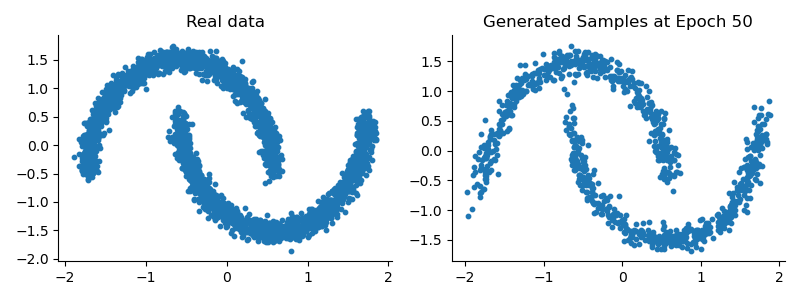
\includegraphics[width=0.8\textwidth]{./figures/samples_epoch50}
    \end{figure}
    
\end{enumerate}